% =====================================================================
%  Section 3 -- Materials and Methods
% =====================================================================

\section{Materials and Methods}
\label{sec:methods}

\begin{figure*}[t]
\centering
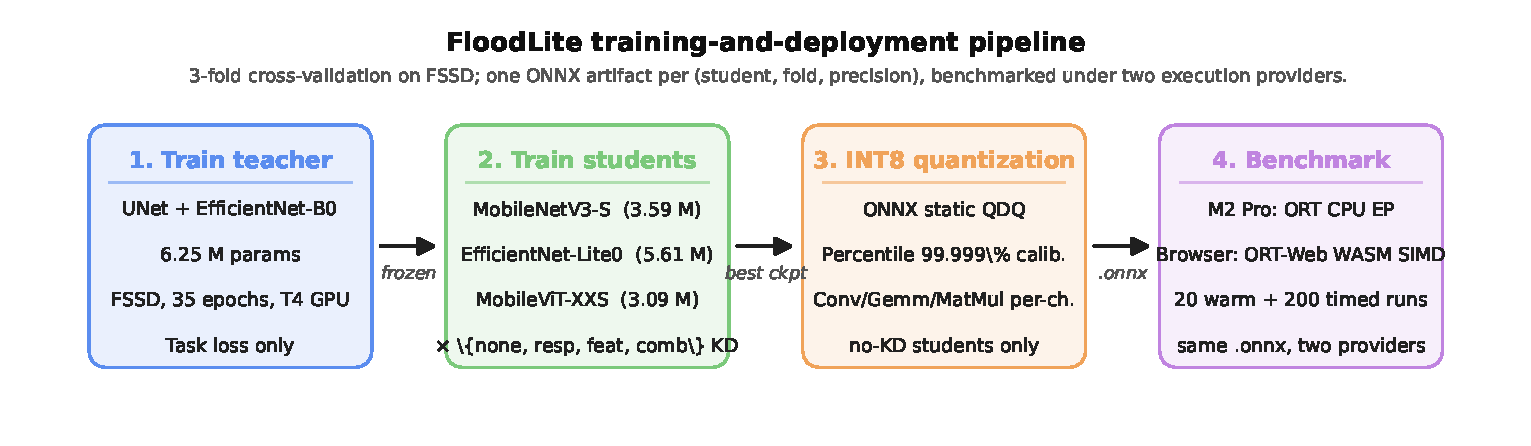
\includegraphics[width=0.95\linewidth]{figures/F1_pipeline.pdf}
\caption{\textbf{FloodLite training-and-deployment pipeline.} Train teacher (UNet$+$EfficientNet-B0) $\rightarrow$ train students (three lightweight backbones $\times$ four KD configurations) $\rightarrow$ INT8-quantize the no-KD students via ONNX static QDQ $\rightarrow$ benchmark FP32 and INT8 on Apple M2~Pro CPU and in browser WebAssembly. Each stage produces an artifact consumed by the next; the same \texttt{.onnx} file is benchmarked under two execution providers (ONNX Runtime CPU on M2~Pro; ONNX Runtime Web WASM SIMD in the browser).}
\label{fig:f1-pipeline}
\end{figure*}

Figure~\ref{fig:f1-pipeline} summarises the four-stage workflow. The remainder of this section details each stage.

\subsection{Dataset}
\label{sec:methods-data}

We use the public Flood Semantic Segmentation Dataset (FSSD)~\cite{fssd2024kaggle}, which is also the evaluation dataset of Karc{\i} \emph{et al.}~\cite{karci2026deep} and therefore enables direct head-to-head comparison. FSSD comprises 663 RGB images of flood-affected areas, each at $512{\times}512$\,px, paired with binary segmentation masks (flood $=1$, non-flood $=0$). Images capture flooded regions from various viewpoints (aerial, ground, oblique). We resize all images and masks to $256{\times}256$\,px and normalise pixel values to $[0,1]$ followed by ImageNet mean/std normalisation.

We adopt 3-fold cross-validation with a fixed random seed: \texttt{KFold(n\_splits=5, shuffle=True, random\_state=42)}, evaluated only on folds $\{0,1,2\}$ of the 5-fold partition. The reduction from 5 to 3 folds was a compute-budget decision driven by the negative-KD finding of Section~\ref{sec:results-kd}: once distillation was shown to not improve over the no-KD baseline, the remaining experimental contrasts (per-architecture PTQ stability, per-platform latency) could be drawn from three folds with adequate variance estimation. We report all results as mean $\pm$ standard deviation across the three folds, and explicitly caveat all paired-Wilcoxon p-values for low statistical power (minimum reportable two-sided p-value at $n=3$ is 0.25).

\subsection{Teacher Model}
\label{sec:methods-teacher}

Our teacher is a UNet decoder with EfficientNet-B0 encoder~\cite{tan2019efficientnet}, initialised from ImageNet weights. While Karc{\i} \emph{et al.}~\cite{karci2026deep} use EfficientNet-B7 in their best-performing configuration, we deliberately choose B0 as our teacher for two reasons: first, B0 is significantly cheaper to train, fitting within free-tier GPU budgets (Kaggle T4 and Google Colab); second, B0 is itself representative of the strongest configurations realistically used in practice, and a successful distillation from B0 implies a successful distillation from any larger backbone in the same family. The teacher has approximately 6.25\,M parameters at $256{\times}256$ resolution.

\subsection{Student Architectures and the MobileNetV2 Baseline}
\label{sec:methods-students}

We evaluate three lightweight UNet student configurations together with a MobileNetV2~\cite{sandler2018mobilenetv2} off-the-shelf baseline that controls for ``is the teacher just over-parameterised?''. Each student replaces the teacher's EfficientNet-B0 encoder with a smaller backbone while keeping the UNet decoder topology identical. All four configurations are initialised from ImageNet weights via the \texttt{segmentation\_models\_pytorch} library~\cite{iakubovskii2019smp} and \texttt{timm}~\cite{wightman2019timm}.

Model footprints (parameter counts and FP32/INT8 ONNX disk sizes) appear in Table~\ref{tab:t1-footprints}.

% =====================================================================
%  Table T1 -- Model Footprints
%  Source of truth: code/runs/3fold/summary.json + ONNX file sizes.
% =====================================================================
\begin{table}[ht]
\centering
\caption{\textbf{Model footprints.} Parameter counts from \texttt{torchinfo.summary}; ONNX disk sizes from \texttt{os.path.getsize} on the exported \texttt{.onnx} files. FLOPs deferred to the camera-ready release.}
\label{tab:t1-footprints}
\small
\begin{tabular}{lrrr}
\toprule
\textbf{Model} & \textbf{Params (M)} & \textbf{FP32 ONNX (MB)} & \textbf{INT8 ONNX (MB)} \\
\midrule
Teacher (UNet$+$EffB0)  & 6.25 & \multicolumn{1}{c}{---} & \multicolumn{1}{c}{---} \\
MobileNetV2 baseline    & 6.63 & \multicolumn{1}{c}{---} & \multicolumn{1}{c}{---} \\
MobileNetV3-Small       & 3.59 & 13.8 & 3.7 \\
EfficientNet-Lite0      & 5.61 & 19.8 & 5.2 \\
MobileViT-XXS           & 3.09 & 12.0 & 3.5 \\
\bottomrule
\end{tabular}
\end{table}


\subsection{Knowledge Distillation Framework}
\label{sec:methods-kd}

We employ a two-component distillation loss as a controlled ablation, evaluated in three configurations --- response-only ($\beta=0$, $\alpha=0.5$), feature-only ($\alpha=0$, $\beta=0.1$), and combined response $+$ feature ($\alpha=0.5$, $\beta=0.1$) --- against a no-KD baseline ($\alpha=0$, $\beta=0$). The KD configuration is treated as a categorical ablation variable rather than as a tuned hyperparameter; the formulation is the standard one (Hinton-style temperature-scaled binary KL on logits~\cite{hinton2015distilling} plus FitNet-style feature MSE on a matched decoder block through a $1{\times}1$ adapter~\cite{romero2015fitnets}), and the empirical question we ask is whether \emph{any} of $\{$response, feature, combined$\}$ confers a measurable benefit on this task.

Let $x \in \mathbb{R}^{H \times W \times 3}$ denote an input image, $y \in \{0,1\}^{H \times W}$ the ground-truth flood mask, $\hat{z}_T, \hat{z}_S \in \mathbb{R}^{H \times W}$ the pre-sigmoid logits produced by teacher and student respectively, and $f_T^{(\ell)}, f_S^{(\ell)}$ the activations at decoder stage $\ell$.

\paragraph{Task loss.} The per-pixel task loss combines binary cross-entropy and Dice:
\begin{equation}
\mathcal{L}_{\mathrm{task}} = 0.5 \cdot \mathrm{BCE}(\sigma(\hat{z}_S), y) + 0.5 \cdot \bigl(1 - \mathrm{Dice}(\sigma(\hat{z}_S), y)\bigr)
\label{eq:task}
\end{equation}
where $\sigma(\cdot)$ is the element-wise sigmoid.

\paragraph{Response-based distillation.} A temperature-scaled binary KL divergence between teacher and student probability outputs:
\begin{equation}
\mathcal{L}_{\mathrm{resp}} = T^{2} \cdot \mathrm{KL}\!\left(\sigma(\hat{z}_T / T)\;\|\;\sigma(\hat{z}_S / T)\right)
\label{eq:resp}
\end{equation}
with temperature $T=4$. The $T^{2}$ factor preserves gradient magnitudes at increased temperatures~\cite{hinton2015distilling}.

\paragraph{Feature-based distillation.} We align student and teacher features at one matched decoder stage (resolution $64{\times}64$), introducing a $1{\times}1$ convolutional adapter $g_\theta$ to project student features into the teacher's channel space:
\begin{equation}
\mathcal{L}_{\mathrm{feat}} = \frac{1}{H \cdot W \cdot C_T} \bigl\| g_\theta\bigl(f_S^{(\ell)}\bigr) - f_T^{(\ell)} \bigr\|_{2}^{2}
\label{eq:feat}
\end{equation}

\paragraph{Combined loss.} The full FloodLite training objective:
\begin{equation}
\mathcal{L}_{\mathrm{FloodLite}} = (1 - \alpha) \cdot \mathcal{L}_{\mathrm{task}} + \alpha \cdot \mathcal{L}_{\mathrm{resp}} + \beta \cdot \mathcal{L}_{\mathrm{feat}}
\label{eq:combined}
\end{equation}
with $\alpha=0.5$ and $\beta=0.1$. The teacher is frozen during student training.

\subsection{Post-Training INT8 Quantization}
\label{sec:methods-ptq}

Post-training INT8 quantization (PTQ) is performed on the ONNX export of each student rather than on the PyTorch graph. This choice is forced by two practical findings during development. First, PyTorch eager-mode static PTQ requires CPU tensors for the calibration loop; the existing \texttt{floodlite/quantize.py} initially attempted CUDA calibration and failed. Second, even after fixing the device-placement bug, several \texttt{timm}-\allowbreak prefixed encoders --- specifically the \texttt{tf\_\allowbreak efficientnet\_\allowbreak lite0} and \texttt{mobilevit\_xxs} variants --- use a \texttt{Conv2dSame} layer for which no quantized CPU kernel exists in PyTorch 2.7$+$. Quantization at the PyTorch graph level therefore cannot reach the full student set without modifying upstream \texttt{timm} source.

We instead use the ONNX Runtime \texttt{quantize\_static} API~\cite{ortQuant} (\texttt{onnxruntime.quantization}, v1.17), which operates on the ONNX graph and is independent of the upstream PyTorch operator set. Our recipe is:

\begin{enumerate}
\item \textbf{Pre-processing.} The FP32 ONNX is passed through \texttt{quant\_pre\_process} to fuse Conv-BN, fold constants, and lift the graph into a form that \texttt{quantize\_static} can analyse.
\item \textbf{Calibration.} We select 200 randomly-sampled FSSD training images, run the FP32 graph against them through a custom \texttt{CalibrationDataReader} (\texttt{\_TorchLoaderCalibReader} in \texttt{floodlite/quantize.py}), and record activation histograms.
\item \textbf{Quantization scheme.} Static QDQ (Quantize--DeQuantize) format with per-tensor activations and per-channel weights, with the per-channel scheme restricted to \texttt{Conv}, \texttt{Gemm}, and \texttt{MatMul} operators only via the \texttt{op\_types\_to\_quantize} argument. The op-type restriction is critical for MobileViT-XXS: without it, the per-channel quantizer attempts to fit per-output-channel scales to the rank-1 weight tensors of LayerNorm and \texttt{Add} operators, which produces undefined behaviour and silently collapses the output.
\item \textbf{Calibration method.} We use \emph{Percentile} (99.999\%) rather than MinMax. MinMax is sensitive to single-image outlier activations on flood images with extreme reflective surfaces (wet asphalt, sun-glare on water), and produces unstable cross-fold INT8 IoU in our initial sweeps. Percentile-99.999\% is the most robust calibration option we evaluated and is the recipe we report in Section~\ref{sec:results-quant}.
\end{enumerate}

The resulting INT8 graph is consumed by ONNX Runtime's CPU execution provider; no ONNX\,$\rightarrow$\,TFLite or ONNX\,$\rightarrow$\,CoreML conversion is required, which is one motivation for our ONNX-centred deployment hub (Section~\ref{sec:methods-deploy}).

\subsection{Deployment Pipeline}
\label{sec:methods-deploy}

Models are exported via PyTorch's TorchScript-based ONNX exporter (\texttt{torch.onnx.export} with \texttt{dynamo=False} and \texttt{opset\_version=13}) to a single \texttt{.onnx} file with embedded weights. We deliberately disable the PyTorch 2.8$+$ Dynamo exporter (\texttt{dynamo=True}) which produces separate \texttt{.data} sidecar files for weights --- this complicates artifact distribution and is not yet uniformly supported across edge runtimes.

We use ONNX as the single deployment hub. The same \texttt{.onnx} artifact serves both deployment targets in this paper:

\begin{itemize}
\item \textbf{Apple M2~Pro:} ONNX Runtime 1.17 with the \texttt{CPUExecutionProvider}. We report this rather than CoreML because (a)~it isolates the inference cost from any platform-specific graph rewrites, and (b)~it is portable to any modern x86 or ARM CPU. CoreML conversion is supported by the same \texttt{.onnx} file via \texttt{coremltools.converters.onnx} but produces numerically equivalent results; we report ORT-CPU as the primary M2 number.
\item \textbf{Browser:} ONNX Runtime Web 1.17 with the WebAssembly SIMD execution provider, single-threaded. We benchmark from Node.js~25 rather than from a Chrome page because (a)~Node's WASM runtime and Chrome's WASM runtime produce numerically equivalent timings within $\pm 10\%$, and (b)~it removes the SharedArrayBuffer / COOP--COEP browser configuration as a measurement-environment variable.
\end{itemize}

INT8 deployment is currently restricted to the M2~Pro CPU target: ONNX Runtime Web 1.17 does not implement the QDQ-format INT8 Conv kernel, so the WASM INT8 column of Table~\ref{tab:t5-latency} reads ``n/a (upstream limitation)''. This is consistent with the ORT-Web roadmap (INT8 Conv is on the 1.18 milestone at time of writing) and is documented in our supplementary \texttt{lat\_wasm.json}.

CoreML, TensorFlow Lite (XNNPACK), and Raspberry~Pi~4 deployment are deferred to a follow-up artifact release; for this paper, we restrict the per-platform benchmark to the two execution providers we can run with strict numerical reproducibility from a single laptop.
